\section{The robotic platform}
\label{sect:robot}

\begin{figure}
\centering
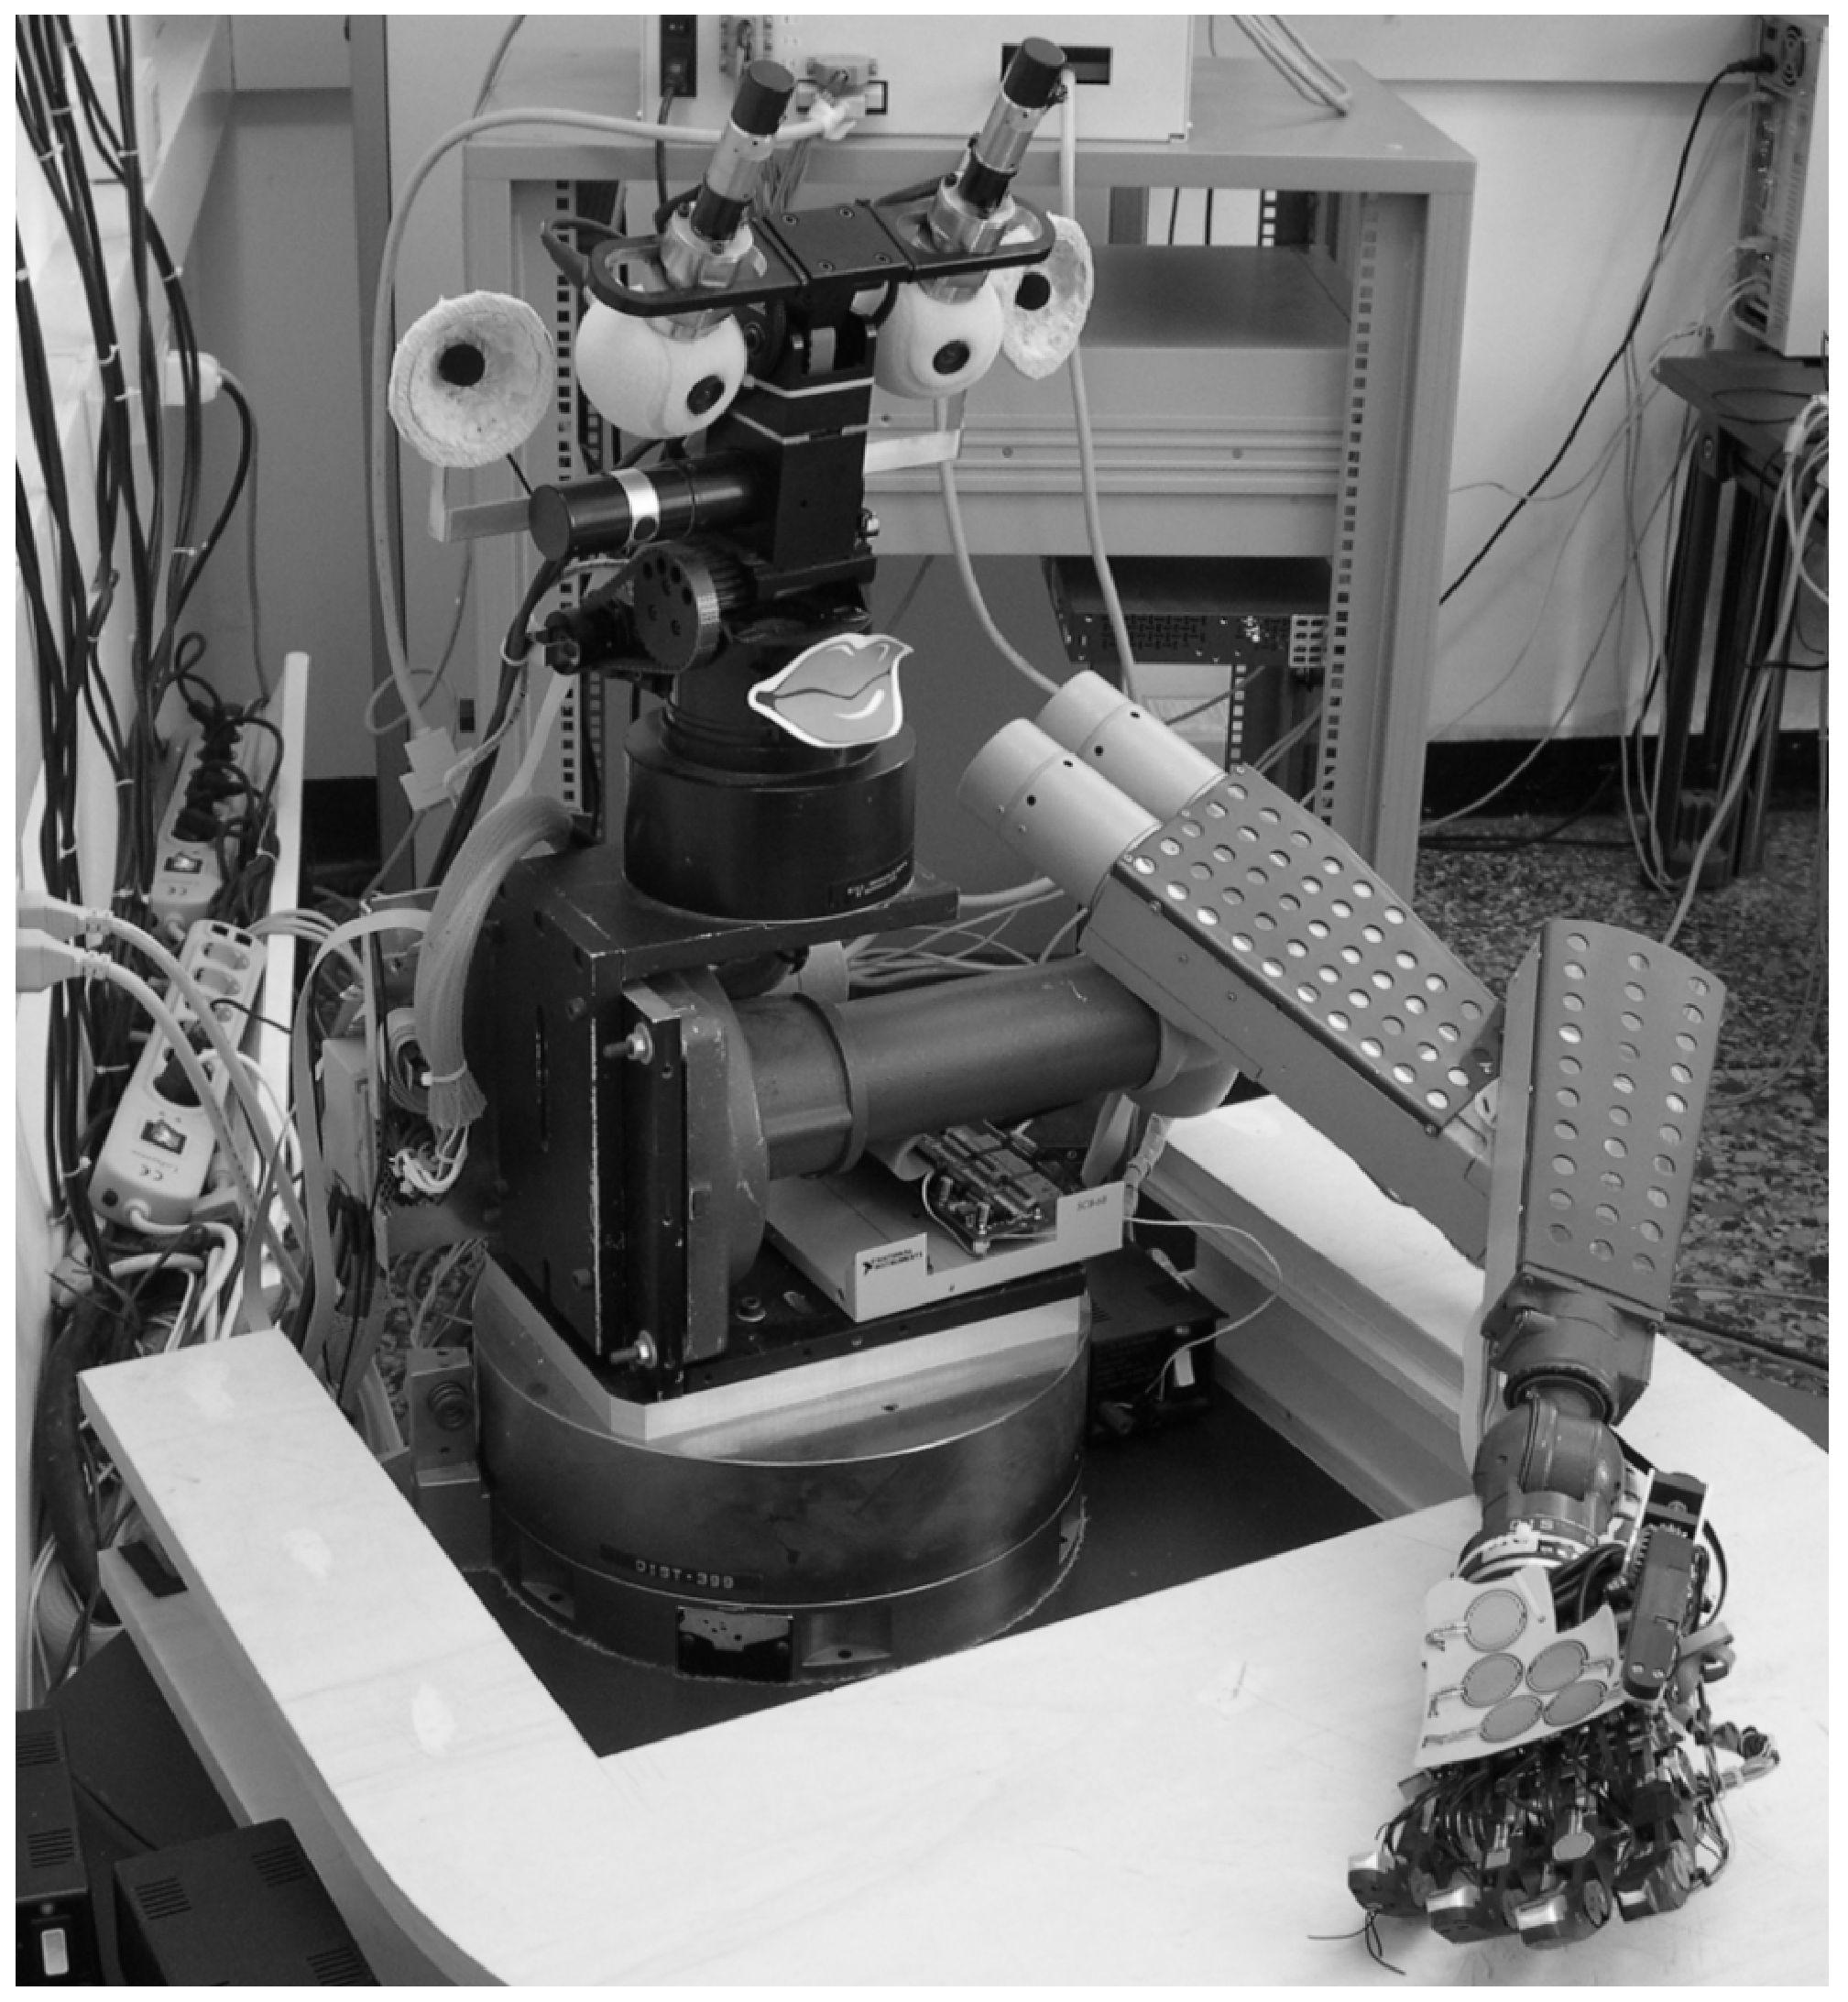
\includegraphics[width=3in]{robot1}
\caption{The robotic platform: The Babybot.}
\label{fig-platform}
\end{figure}

The experiments reported in this paper were performed by using an upper torso humanoid robot called Babybot (Figure~\ref{fig-platform}). The Babybot consists of a head, an arm and a hand. The head has five degrees of freedom, and it is equipped with two cameras, two microphones and a set of gyroscopes. The cameras can pan independently and tilt around a common axis; the remaining degrees of freedom allows the head to pan and tilt at the level of the neck. The arm is an industrial PUMA 260 manipulator. The hand is mounted on the arm end point. It consists of a total of 16 degrees of freedom actuated by only 6 motors. Its five fingers are thus largely underactuated: the thumb and index are controlled independently by two motors each, whereas the remaining two motors are connected to the middle, ring and small finger which form a single virtual joint. The coupling between each joint and the motors is achieved by means of springs which give the hand a certain degree of compliance and elasticity. Magnetic potentiometers provide position and force feedback at each joint whereas force sensing resistors on the palm and fingers provide tactile feedback (see figure~\ref{fig-platform} and figure~\ref{fig-platform2}). A more detailed description of the hand can be found in \cite{natale04thesis}.

\begin{figure}
\centering
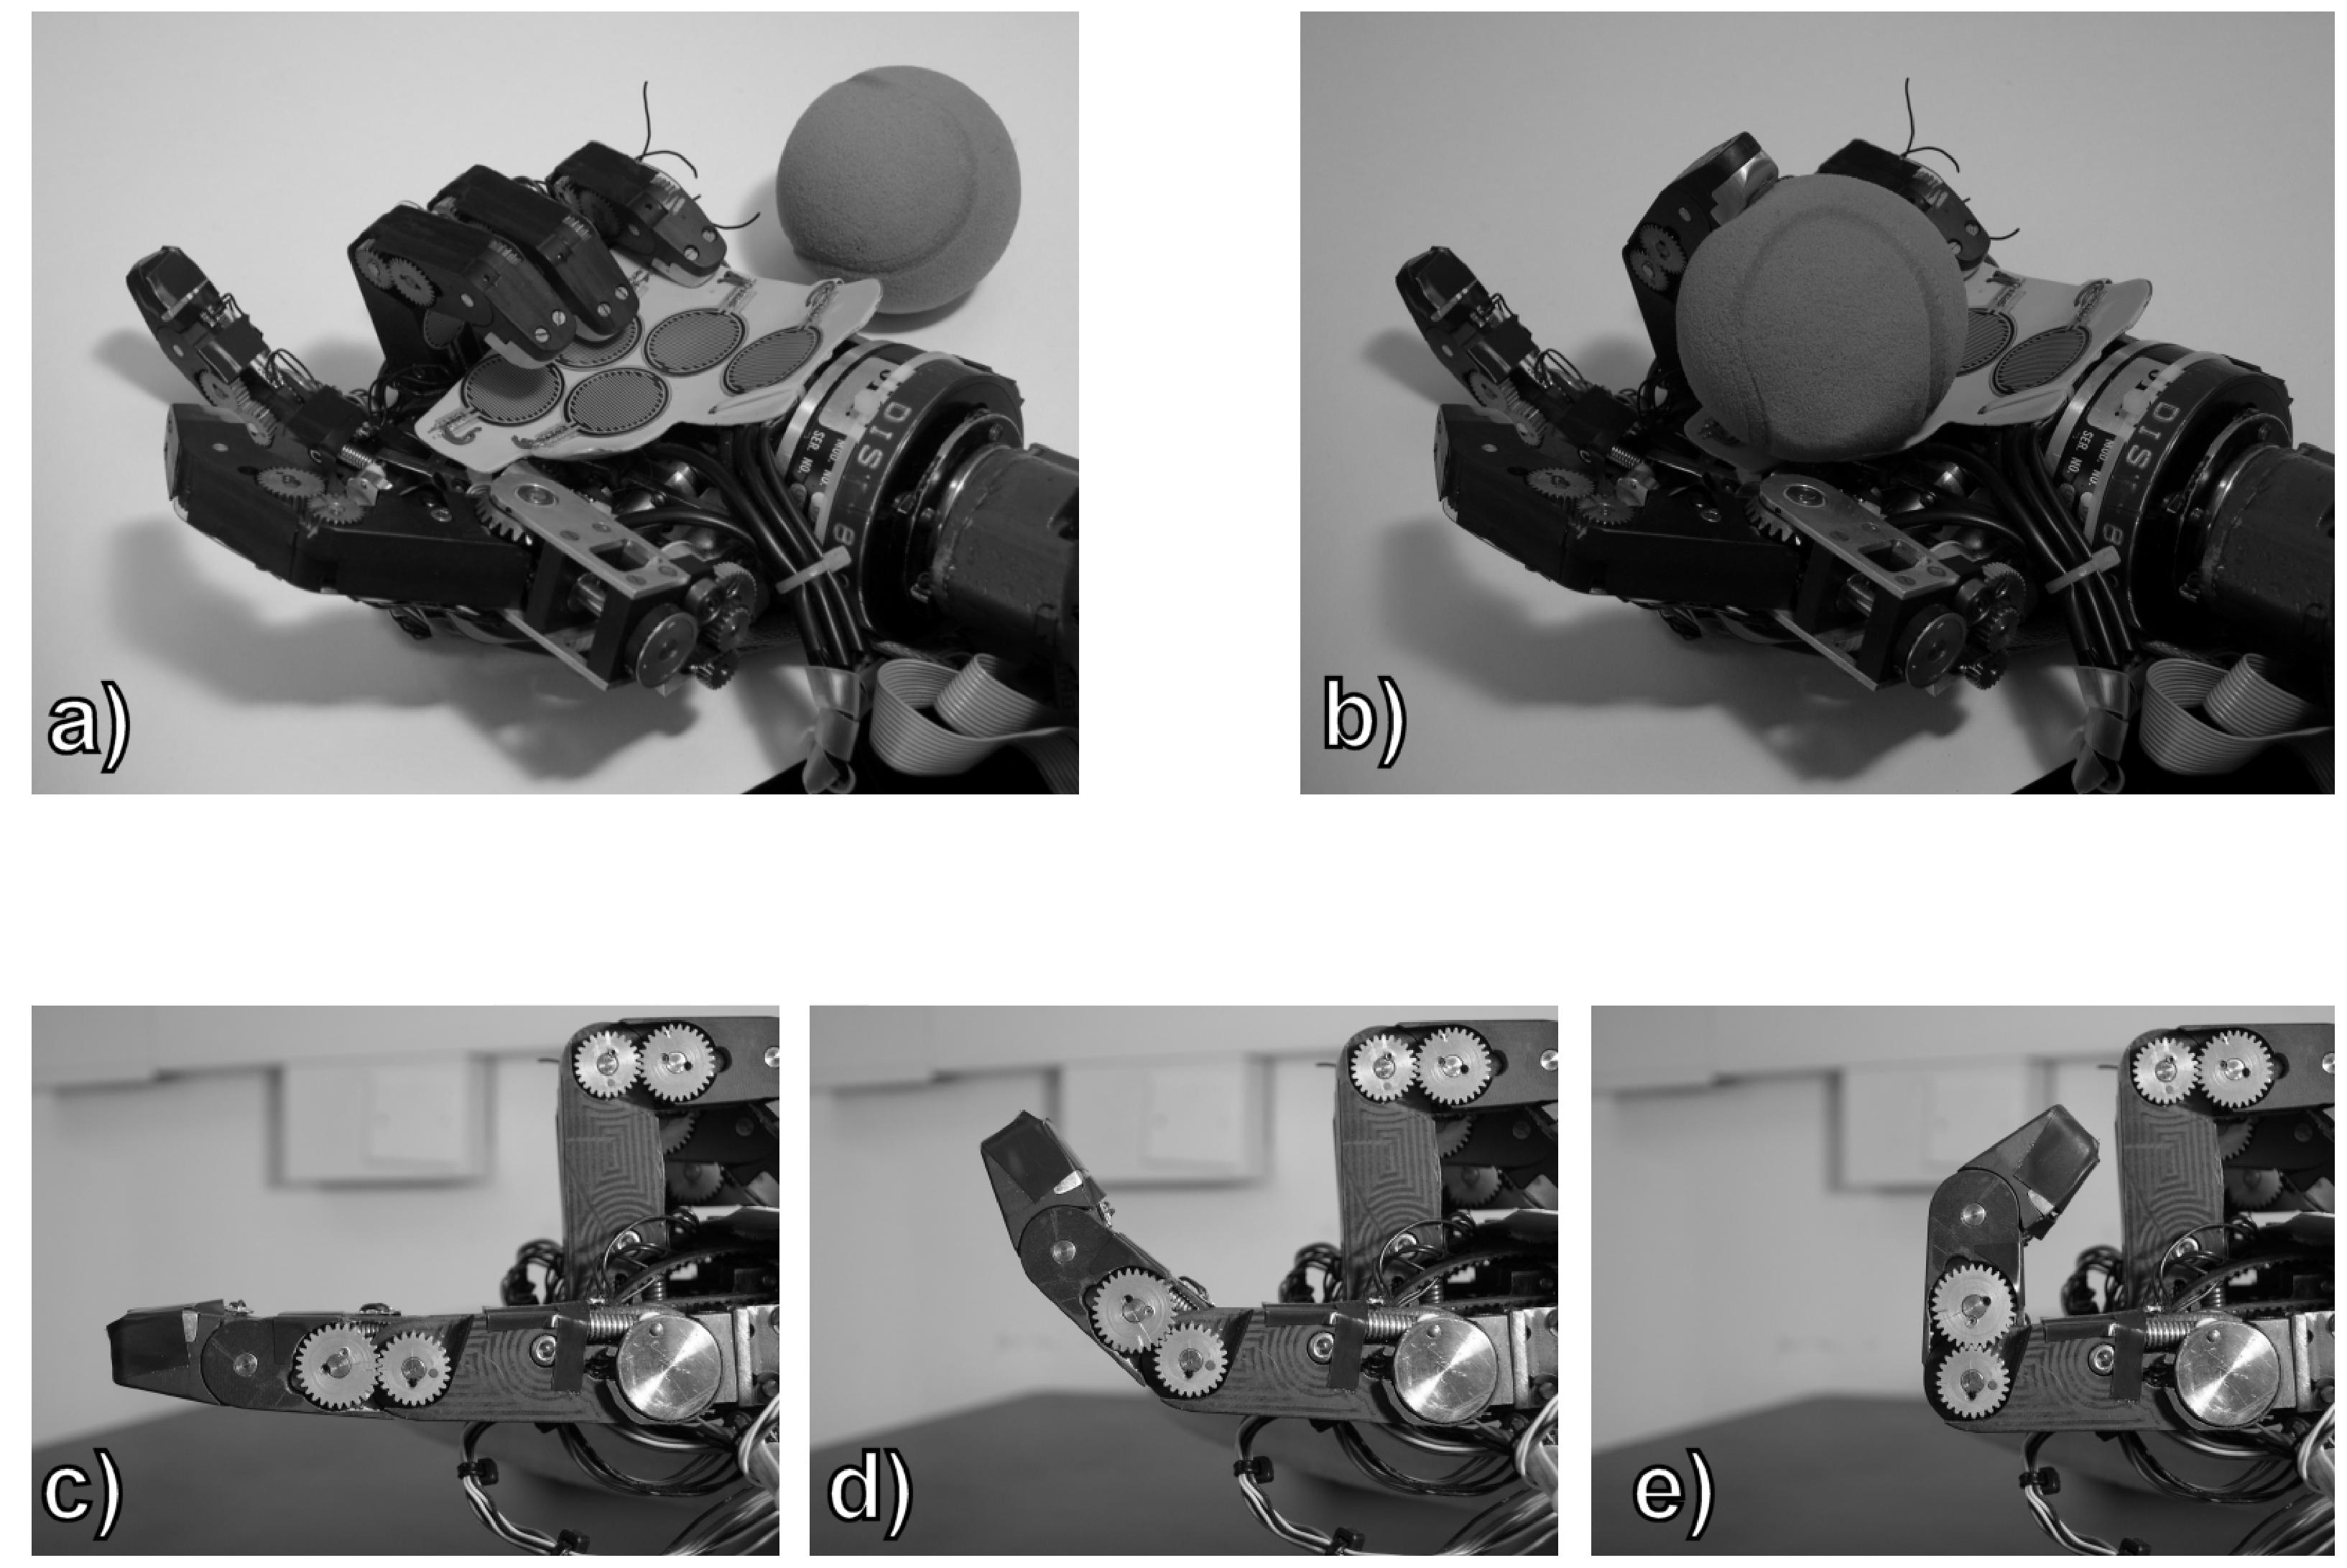
\includegraphics[width=3in]{robot2}
\caption{Details of the hand of the Babybot.}
\label{fig-platform2}
\end{figure}

